\section{Design and operation of the second generation of interferometric gravitational wave detectors}\label{subsec:2ndgen}

Even while the initial LIGO and Virgo detectors were still far from their design sensitivities, plans were afoot for major upgrades to each, aimed at achieving roughly a factor 10 improvement in sensitivity over the whole frequency band. 
This generation of detectors would be known as the 2nd generation, or the advanced detectors; Advanced LIGO\cite{Aasi_2015b,aLIGOSensitivity} and Advanced Virgo\cite{aVirgoTR2012}. 

Besides generally targeting a factor 10 overall improvement in sensitivity, and an expansion of the sensitive frequency band towards lower frequencies, the design of the advanced detectors was aimed at making them limited by fundamental noises: thermal noise and quantum noise (acombination of quantum radiation pressure noise and laser shot noise).
As a consequence, all other possible sources of noise needed to be pushed well below these main ones.
As an example, \autoref{fig:aLIGOnbudget} shows the main contributions to the Advanced LIGO design noise budget, together with the seinsitivity of the Hanford and Livingston detectors during their first observing run.

Given the many similarities between the LIGO and VIRGO projects, and the fact that, at the time of writing, Advanced Virgo is still in the process of installing upgrades and commissioning, in this chapter we will concentrate on a description of the Advanced LIGO layout and main subsystem, highlighting the most relevant differences with Advanced Virgo.

\begin{figure}[htb]
	\begin{center}
		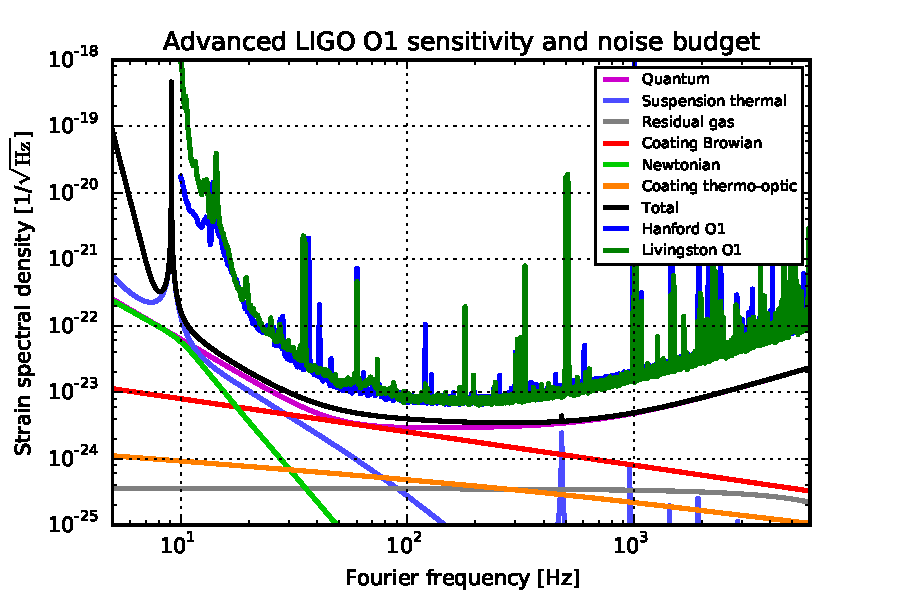
\includegraphics[width=0.9\textwidth]{Figures/aLIGOnbudget.pdf}
		\caption{\label{fig:aLIGOnbudget}Predicted strain equivalent spectral densities for major noise sources in Advanced LIGO at full input laser power. Also shown are the typical strain sensitivities of the Hanford and Livingston detectors throughout the O1 run, from September 2015 to January 2016, during which the first direct detection of gravitational waves was made.}
	\end{center}
\end{figure}

\subsection{Suspensions and seismic isolation.}
While the Virgo superattenuator test-mass suspensions, described in \autoref{sec:Virgo}, already performed extremely well and only required minimal modifications, two of the subsystems that were most significantly upgraded from LIGO to Advanced LIGO were the Seismic Isolation\cite{SEI2015} and Suspension subsystems.
Although they are formally two separate subsystems, they work in concert to isolate the test-masses and  other critical optics from ground vibrations and other macroscopic motions, and ensure that the they can move as free masses in the relevant degree of freedom above a few Hz.

In Advanced LIGO, the test masses are suspended by four-stage pendula, known as the quad suspensions\cite{Aston_2012}. 
From top to bottom, the main suspension chain is composed of two metal masses, and two 40\,kg cylindrical fused silica substrates
of 34\,cm diameter and 20\,cm thickness, the lowermost one being the test mass.
The first metal mass is attached to the suspension structure by four blade springs providing vertical isolation;
a steel wire runs from the tip of each blade to the 
suspended mass.
In a similar fashion, the second metal mass is attached to the first one, 
and so is the penultimate mass; itself actually a fused silica substrate of equal dimensions to the test masses themselves. 
In the final stage of the suspension, however, the test mass 
is attached to the penultimate mass by four fused silica fibers; these are directly welded to 
the two optics to form a monolithic assembly.
The monolithic suspension design offers reduced mechanical losses, and
consequently lower thermal noise, than the previously used metal wire suspensions.
The pendulum resonances of the four stages are 
distributed between 1 and 4 Hz, providing a passive suppression of motion along 
the optical axis by $10^7$ at 10\,Hz and improving as the frequency to the eighth power.

A similar chain of masses called the reaction chain hangs parallel to the main one, 
and supports the sensors and actuators used for local damping and active positioning and alignment control 
of the lowermost three masses of the main chain. The reaction chain provides a quiet reference point 
for the control forces.
The top masses of both chains are instead actuated using the suspension structure as a reference.
For all stages except the lowest, the sensors/actuators are compact units that use shadow sensors to measure the position of, and electromagnets to exert forces on, permanent magnets attached to the masses.
The last stage has no local sensors, since the position of the test mass is sensed 
by the global interferometry; on the end test mass, the actuators consist of patterns of electrodes 
deposited on the last mass of the reaction chain, which exert electrostatic forces on the test mass when polarized.
This avoids the need of attaching magnets to the test masses, thus maintaining low mechanical 
losses and reducing possible couplings to external fields.
The last stage of the reaction chain on the input test mass suspension has no actuators at all, and is instead used as the \textit{compensation plate} for the thermal compensation system.

Each quad suspension is attached to an in-vacuum seismic isolation platform, 
used for further suppression of ground vibrations and precise positioning and 
alignment with a larger range than allowed by the suspensions themselves. The 
platforms are six-axis, with two-stage active and passive isolators proving more 
than 3 orders of magnitude isolation above 1\,Hz, and positioning capabilities 
with nm resolution over a range of several mm.

Similar seismic isolation platforms are used to support all the in-vacuum optics; 
the optics that are part of an optical cavity are further suspended by triple-pendula, while 
single-pendulum suspensions, or specialized geometries, are used to isolate 
less critical optics where necessary.

In both the Hanford and Livingston Advanced LIGO detectors, 
each of the in-vacuum seismic isolation platforms is 
installed on beams that are decoupled from the vacuum system itself via 
flexible bellows, and supported from the outside using hydraulic actuated 
piers anchored to ground.
This system acts as a further layer of isolation and is used to predictively correct for macroscopic positioning drifts caused by tidal forces from the moon and the sun.

	
\subsection{Laser}
At frequencies above about 100\,Hz, the interferometer sensitivity is limited by shot 
noise in the laser. The relative impact of the shot noise scales as the inverse of the 
square root of the power: increasing the laser power is thus a conceptually 
straightforward way of improving the sensitivity in the shot-noise limited band. 
The Advanced LIGO laser source is designed to deliver a maximum of 180\,W of laser power, as opposed to the 35\,W used in eLIGO.
In order to achieve this goal the laser source is composed of a 2\,W Nd:YAG 1064\,nm non-planar ring oscillator (NPRO) master laser, amplified up to 35\,W by a single-pass medium-power amplifier, subsequently amplified to 220\,W by an injection-locked ring ring oscillator known as the high-power oscillator stage~\cite{Kwee_2012}. 

This beam is then pre-stabilized in frequency with respect to a fixed spacer cavity in a thermally shielded environment, and pre-stabilized in intensity with respect to several reference photodiodes. 
The beam from the pre-stabilized laser is also passed through a pre-mode cleaner ring cavity, which filters the spatial mode of the laser ensuring a high-purity Gaussian beam profile. 
The beam is then handed off to the Input Optics subsystem, where phase modulation sidebands are applied and the power of the beam is controlled, before the beam is passed to the in-vacuum suspended input mode cleaner cavity~\cite{Mueller_2016}. 
This cavity serves to further filter the beam in both frequency and spatial mode, passively suppressing any beam jitter of the pre-stabilized laser beam from non-isolated optical components. 
The beam transmitted from the input mode cleaner is then passed through a Faraday isolator, before being expanded and matched to the 
main interferometer mode.

Advanced Virgo employs a similar system, although with a slightly different technological implementation, to deliver up to 125\,W into the main interferometer. Despite the lower input power, the circulating power in the arm cavities in about the same as in Advanced LIGO, due to different gains in the power recycling and arm cavities.

\subsection{Thermal compensation system}
Despite the stringent requirements on the optical absorption of bulk and coating 
material of the optics, the high power levels circulating in the interferometer result 
in a non-negligible amount of heat deposited into the optics.
Due to the poor heat conduction in vacuum, this induces important thermal gradients that can modify 
the optical parameters of the system via two main effects: thermal lensing in the 
bulk material due to the temperature dependence of the refractive index,
and distortion of the high reflectivity (HR) surface of the mirrors due to thermo-mechanical stress.
HR surface distortion is particularly important for the input and end test masses, both because they see the highest power level of all the interferometer optics (up to about 1\,MW), and because any deformation of their surface has a bigger impact on the interferometer output.
Thermal lensing, while irrelevant for the end test mass due to the secondary role of the weak transmitted diagnostic beam, is an important effect in the input test masses, since it can spoil both the mode matching with the power recycling cavity and the mode overlap between the two arm cavities, thus decreasing the overall contrast of the interferometer.

The Advanced LIGO thermal compensation system is designed to monitor and compensate for both effects across the entire range of operating powers, and constitutes a substantial improvement over the much simpler implementation used in eLIGO.
To sense the thermal distortion, each of the four input and end test masses is monitored using a custom Hartman wavefront sensors, which uses an auxiliary superluminescent diode beam injected from the anti-reflection face of the optic and reflected back from the HR side (thus traversing the optic twice).
To correct for HR surface distortions, an infrared annular heater heats the barrels of the test masses, reducing the thermal gradient and inducing a thermal stress that counteracts the effect of the central heating due to the main laser beam.
Finally, a CO$_2$ laser projector is used to impress a suitable pattern on the compensation plate, deliberately creating a thermal lens that compensates for the lens left in the input test mass after the combined effects of the science beam and the annular heater~\cite{TCS_inpreparation}.

The main difference in the Advanced Virgo implementation of the Thermal Compensation System is the addition of a scanning CO2 projector, which compared to a fixed-mask one promises greater flexibility and adaptability of the shape of the projected pattern.

\subsection{Optical layout}
The optical layout of Advanced LIGO is different from the initial LIGO layout in several ways. 
The most fundamental change to the optical layout is the addition of a signal recycling 
mirror between the anti-symmetric side of the beam splitter and the optical detection port. 
In its current configuration this oft-called signal recycling mirror is actually tuned such as to 
increase the bandwidth of the detector, rather than increasing the quantum noise-limited sensitivity
in a narrow band as the name \textit{recycling} implies. As such, a more apposite name for this mirror 
in the current configuration is signal \textit{extraction} mirror. 

The signal extraction mirror forms a new cavity within Advanced LIGO; which is still called the signal recycling cavity. 
Both the signal recycling cavity and the power recycling cavity in Advanced LIGO are designed to be 
geometrically \emph{stable}, by which it should be understood that the round-trip Gouy phase in the cavity 
is significant, and thus higher-order spatial modes are non-degenerate~\cite{Arain2008}. 
This is in contrast to the power recycling cavity in initial LIGO, which was only marginally stable. 
The advantages of the stable recycling cavity design have been clear during the commissioning of 
Advanced LIGO, where commissioning of the length and alignment sensing and control systems has 
been a much smoother process than in initial LIGO. 

Another important geometric change to the optical layout between initial LIGO and Advanced LIGO is 
in the arm cavities. There was a drive towards using larger beam spot sizes on the mirrors in Advanced 
LIGO in order to mitigate the effects of thermal noise. In general there are two cavity geometry solutions available 
that will give a specific beam spot size on the mirrors for a two-mirror cavity of fixed length. The initial LIGO 
arm cavities were designed with a large beam waist inside the cavities
whereas Advanced LIGO uses the alternative solution of having a small beam waist size in the cavities. 
The major advantage to the small beam waist size solution is that thermal deformations of the test masses caused by 
absorption in the coatings push the cavity to a more stable geometry, rather than towards a less stable geometry as 
is the case for the large beam waist design. 

Several additional optical subsystems have been added in the upgrade from initial LIGO to Advanced LIGO. 
During the enhanced LIGO phase (shortly before initial LIGO went offline for the major upgrade to aLIGO) an output
mode cleaner was added at the output port. The output mode cleaner is a crucial component of the DC readout 
scheme which was first demonstrated in GEO600, and which was determined to be a more optimal solution for 
readout of the gravitational wave signal than the previously used RF heterodyne readout scheme~\cite{DCreadout}. The output mode cleaner subsystem was retained in the aLIGO optical layout, and takes the form of a suspended fixed spacer cavity with a bow tie configuration.
The output mode cleaner has the essential function of removing RF sidebands and higher-order spatial modes from the light incident on the photodiode, thus mitigating their impact on the shot noise sensitivity. 

A great effort was made in the upgrade to Advanced LIGO to make the lock acquisition process more deterministic than stochastic.
Part of this effort was the inclusion of the arm length stabilization (ALS) subsystem.
This subsystem uses green frequency-doubled Nd:YAG beams which are phased locked to the main laser to independently control the arm cavities during lock acquisition of the central dual-recycled Michelson interferometer (DRMI)~\cite{Staley2014}.
Once the DRMI is locked the ALS can be used to methodically bring the arms to resonance, bringing the full interferometer to the ideal operating point. 
The arm length sensing can be handed off to the main interferometric sensors, once the ALS has brought the interferometer within their linear range.

The optical layout of Advanced Virgo is very similar to that of Advanced LIGO, although restrictions in available vacuum enclosure space prevent the use of stable recycling cavities. In addition, no equivalent of the arm length stabilization system was included int he baseline Advanced Virgo design.

\subsection{Interferometric sensing and control}
The dual-recycled Fabry-P\'{e}rot Michelson interferometer that makes up aLIGO has a very narrow linear range. 
The practical consequence of this fact, when combined with the fact that even with the advanced seismic isolation systems typical 
mirror motions at low frequencies can be of the order several wavelengths, is that length control loops are essential in order 
to keep the interferometer operating with high sensitivity. 

The length sensing of all interferometric ground-based gravitational wave detectors is based on the Pound-Drever-Hall (PDH) laser 
frequency stabilization scheme~\cite{PDH}. 
In this scheme an electro-optic modulator is used to add RF phase modulation sidebands to the laser, 
which are typically non-resonant in an optical cavity when the carrier light is resonant.
When the main light frequency, typically called the carrier frequency, is brought close to resonance in the cavity, 
it picks up a phase shift in reflection of the cavity which is proportional to the difference between its 
frequency and the cavity resonant frequency. The sidebands act as a phase reference for comparison with the 
carrier light, and the total reflected light 
from the cavity is detected with a photodetector and demodulated at the original modulation frequency to give an error 
signal for either the cavity length control or the laser frequency control. 

While the PDH scheme described above refers to the sensing of just one length (or frequency) degree of freedom, 
the core interferometers of 2nd generation ground-based gravitational wave detectors require 5 distinct length degrees of freedom to 
be sensed and controlled. Typically these degrees of freedom are broken down into the following list: common arm length, 
differential arm length (where the gravitational wave signal predominantly appears), Michelson tuning, power recycling cavity length and 
signal recycling cavity length. In reality at least two additional degrees of freedom must be controlled; one each for the input 
and output mode cleaner cavities. This presents a formidable challenge, which was solved for Advanced LIGO by the use of two 
different modulation frequencies, at roughly 9\,MHz and 45\,MHz. The 9\,MHz sidebands are resonant in the power recycling 
cavity only, and experience a dark Michelson fringe. Detectors at various ports demodulated at this frequency typically provide 
good length sensing signals for the arm degrees of freedom, as well as the power recycling cavity length. The 45\,MHz sidebands 
are resonant in both power and signal recycling cavities, and experience a bright Michelson fringe. As a result, the detectors demodulated 
at 45\,MHz provide good sensitivity to signal recycling cavity length and the small Michelson degrees of freedom.

The alignment of optics must also be sensed and controlled in gravitational wave detectors. In aLIGO the sensing is currently achieved using a method 
called differential wavefront sensing, developed by Henry Ward and colleagues~\cite{Morrison1994, Morrison1994b}. 
This method is similar in principle to the PDH length sensing, 
except that quadrant photodectors are used 
instead of single-element photodetectors in order to measure the beats between sidebands and carrier in different spatial modes. An 
alternative method developed by Dana Anderson was used in Virgo, whereby the sideband frequencies were chosen such that higher-order 
spatial modes of the sidebands would be co-resonant in some of the optical cavities with the carrier fundamental mode~\cite{Anderson1984}. 
A detailed description of the alignment requirements of a gravitational wave detector, and a sensing scheme based on the wavefront sensing 
is provided in~\cite{Fritschel1998}.

%\item Sesmic isolation upgrade?
%\item Laser power upgrade
%\item Optical layout
%\item sensing and control
%\item Thermal compensation
%\item signal recyling